
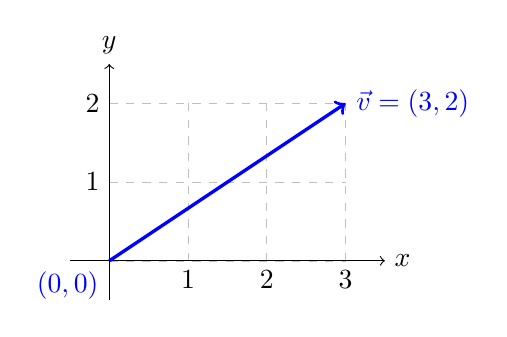
\begin{tikzpicture}
    \draw[step=1,help lines, dashed,lightgray] (0,0) grid (3,2);
    %draw axis value
    \foreach \x in {1,2,3}
        {%
            \draw (\x,0) -- (\x,0) node [below] {$\x$};
        }
    \foreach \y in {1,2}
        {%
            \draw (0,\y) -- (0,\y) node [left] {$\y$};
        }
    %draw lines
    \draw [->] (-0.5,0) -- (3.5,0) node[right]{$x$};
    \draw [->] (0,-0.5) -- (0,2.5) node[above]{$y$};
    \draw [->,blue,very thick] node[below left]{$(0,0)$} (0,0) -- (3,2) node[right]{$\vec{v}=(3,2)$};
\end{tikzpicture}
\captionof{figure}{{\footnotesize 2D vector, $\vec{v}=(3,2)\in{R^2}$}}
\label{fig:vector-and-vector-operation-d1}
